\section{Chatbots}
Ein Chatbot ist ein Programm, das für den Dialog mit Menschen erdacht ist und natürliche Sprache als Text oder Audio entgegennehmen und verarbeiten kann.
Chatbots werden hauptsächlich auf Websites und Instant-Messaging Systemen eingesetzt.
Benutzereingaben werden angenommen und passende Antworten dazu ausgegeben. Außerdem sollen Chatbots Gäste begrüßen und die Unterhaltung in Gang halten.\\
Chatbots können rein regelbasiert oder \acf{KI}-gesteuert reagieren.\\
Durch die inhärente Automatisierung sind Chatbots relevant bezüglich der \glqq{}Unterstützung und Ersetzung von Arbeitskräften\grqq
\footcite[][o. \pno]{Bendel_2018_Chatbot_Definition}{}.
\footcite[Vgl.][o. \pno]{Bendel_2018_Chatbot_Definition}

Chatbots können mit realen Personen oder anderen Chatbots kommunizieren. Ein Chatbot ist jeweils für einen bestimmten Aufgabenbereich vorgesehen und deckt nicht das gesamte Spektrum der menschlichen Kommunikation ab. Ähnlich wie bei Avataren können Chatbots eine \glqq{}körperliche Erscheinung\grqq
\footcite[][71\psq]{de_Vries_2006}
und \glqq{}virtuelle Identität\grqq
\footcite[][71\psq]{de_Vries_2006}
bzw. Charakter haben.
\footcite[Vgl.][71\psq]{de_Vries_2006}

Im Gegensatz zu Agenten arbeiten Chatbots nicht autonom, sondern reaktiv. Sie sind also auf die Befehle von Menschen angewiesen.
\footcite[Vgl.][69\psqq]{de_Vries_2006}

Entscheidend für die Gesprächskompetenz von Chatbots ist das zugrundel iegende Wissen. Die eingesetzten Algorithmen spielen nur eine nachgelagerte Rolle.\\
Für komplexere Problemstellungen  kann es nötig werden, den Kontext genauer zu erfassen. Dazu kann die Gesprächshistorie berücksichtigt und Laufzeitvariablen pro Nutzer gespeichert werden.
\footcite[Vgl.][82\psq]{Feindt_2006_Agenten}

\subsection{Komponenten}
Die wesentlichen Komponenten eines Chatbots sind Utterances (Äußerungen), Intents (Absichten) und Entities (Entitäten).\\
Als Äußerungen gelten alle Eingaben des Nutzers in ihrer Basisausprägung, z. B. \textit{Wie wird das Wetter?}.
Aus der Äußerung wird eine Absicht interpretiert, in diesem Beispiel eine Funktion, die das aktuelle Wetter anzeigt.
Entitäten sind Zusatzparameter für Äußerungen und werden der, mit der Absicht verknüpften Funktion übergeben. Z. B. \textit{Wie wird das Wetter morgen?}, wobei \textit{morgen} die Entität ist.
\footcite[Vgl.][51]{Groetz_2018_Sprich_mit_mir}

\subsection{Arten}
Chatbots werden grundsätzlich als regelbasiert oder selbstlernend kategorisiert.
\footcite[Vgl.][51\psq]{Groetz_2018_Sprich_mit_mir}
\subsubsection{Regelbasiert}
Regelbasierte Chatbots verfügen über einen festen Regelbaum und können nur vordefinierte Fragen beantworten und auf bestimmte Schlüsselwörter reagieren.\\
Wenn der Nutzer sich vertippt, die Fragen leicht anders formuliert oder nicht die richtigen Schlüsselwörter verwendet, kann der Bot daraus keine Aktion ableiten.
\footcite[Vgl.][51\psq]{Groetz_2018_Sprich_mit_mir}
\subsubsection{Selbstlernend}
Durch den Einsatz von \acs{KI} und maschinellem Lernen können Chatbots menschliche Sprache besser verstehen und es muss nicht jede Formulierung eines Satzes angelernt werden. Die Komplexität ist bei dieser Variante höher.
Allerdings können dann Richtigkeit und Qualität der Antworten nicht mehr sichergestellt werden, bzw. die Absicht des Benutzers wird möglicherweise falsch interpretiert.
\footcites[Vgl.][151\psq]{Feindt_2006_Gespraechskompetenz}[Vgl.][51\psq]{Groetz_2018_Sprich_mit_mir}

\subsection{Sonderfall Sprachassistenten}
Als Sonderform der Chatbots können Sprachassistenten betrachtet werden, die sich spätestens seit der Einführung von Amazon Alexa, Google Assistant und Apple Siri großer Beliebtheit erfreuen.
\\
Die Steuerbefehle werden dabei nicht textuell, sondern verbal übergeben und müssen in der Regel durch ein Schlüsselwort wie \textit{Okay Google} oder \textit{Alexa} eingeleitet werden.\\
Dank der Auslagerung der Spracherkennung in die Cloud hat sich die Qualität dieser erheblich verbessert. Das Anlernen von Klangfarbe und Fachvokabular muss nicht mehr individuell manuell vorgenommen werden, sondern geschieht aggregiert in der Cloud.\\
Als zusätzliche Herausforderungen im Vergleich zur textuellen Variante existieren bei Sprachassistenten \glqq{}Dialekte, Sprachfehler und Umgebungsgeräusche\grqq
\footcite[][64]{Puscher_2018_Gut_zugehoert}{}.
\footcites[Vgl.][64]{Puscher_2018_Gut_zugehoert}[Vgl.][50]{Groetz_2018_Sprich_mit_mir}

\subsection{Charakter}
Wichtig für die Akzeptanz eines Chatbots ist, ihm einen Charakter zu verleihen. Es sollte früh entschieden werden, ob er sachlich, empathisch oder frech sein soll.\\
Zu den Eigenschaften zählen Alter, Geschlecht, Erscheinung (Mensch, Tier, Maschine), Zweck und Geschichte bzw. Herkunft.\\
Merkmale wie Humor, Offenheit, Redseligkeit, Auftreten (laut, leise, frech) und Ähnlichkeit mit bekannten Figuren (z. B. Comicfiguren) sollten auch geplant werden.\\
Eine Möglichkeit ist, das Firmenmaskottchen als Chatbot umzusetzen, allerdings sollte abgewägt werden, ob es die nötige Kompetenz verkörpert.
\footcite[Vgl.][68\psq]{Puscher_2018_Gut_zugehoert}




\section{ChatOps}
Der Begriff ChatOps stammt aus dem DevOps-Umfeld und wurde von GitHub durch die Einführung ihres Chatbots \textit{Hubot} im Jahr 2013 geprägt. Jesse Newland, der damals den Vortrag hielt spricht von \glqq{}placing tools
directly in the middle of the conversation\grqq
\footcite[Vgl.][62]{GitHub_2013_Chatops},
also davon, die im Unternehmen genutzten Tools direkt im Chatroom verfügbar zu machen.
\footcite[Vgl.][o. \pno]{Sigler_2014_Chatops}

\subsection{Grundgedanke}
Unter ChatOps wird die Verbindung von Chatbots mit operativen Prozessen verstanden. Dies geschieht durch die transparente Verbindung von Mitarbeitern, Tools, Prozessen und Automatisierung.
Dabei entsteht eine kollaborative Arbeitsumgebung, bei der für alle Mitarbeiter ersichtlich ist, woran gerade wie gearbeitet wird und ermöglicht eine ausführliche Historie der Tätigkeiten und der beteiligten Personen.
\footcites[Vgl.][o. \pno]{Zyane_2017_ChatOps}[Vgl.][190]{Betz_2016_Digital}

Als Grundsatz von ChatOps gilt die \acf{CAMS}, also eine Kultur, die Automatisierung, Messbarkeit und Transparenz mit sich bringt. Dieser Gedanke wurde dem DevOps Umfeld entliehen.
\footcite[Vgl.][o. \pno]{Zyane_2017_ChatOps}

Wenn Fehler auftreten, kann direkt geprüft werden, ob und welche Änderungen am System vorgenommen wurden und nicht alle Mitarbeiter müssen einzeln befragt werden.\\
Auch bei der Einarbeitung von neuen Mitarbeitern ist die Transparenz hilfreich, da sie sämtliche Arbeitsabläufe ihres Teams mitverfolgen können und dazu nicht einmal am gleichen Standort sein müssen. Sie können einfach den Räumen beitreten, die für ihre Rollen und Verantwortlichkeiten vorgesehen sind.
\footcites[Vgl.][o. \pno]{Sigler_2014_Chatops}[Vgl.][66]{Hand_2016_ChatOps}

Durch anpassbare Skripte und Plugins können individuelle Prozesse aus dem Chatroom heraus angestoßen werden. So kann z. B.~in einem Softwareprojekt das Code Deployment gestartet werden oder in der IT-Security auf gemeldete Sicherheitsvorfälle reagiert werden. Außerdem können Benachrichtigungen an die Teammitglieder versendet werden, die gerade zuständig sind.
\footcite[Vgl.][o. \pno]{Sigler_2014_Chatops}

\subsection{Komponenten}
Um ChatOps einführen zu können, müssen als Kernkomponenten ein Kollaborationswerkzeug, ein Bot und eine Systemintegration gegeben sein.\\
Ein Kollaborationswerkzeug ist das Chat-Tool, in dem Stakeholder miteinander kommunizieren können und in Teams organisiert sind.\\
Ein Bot im ChatOps-Kontext bildet die Brücke zwischen Kollaborationswerkzeug und Systemwerkzeugen. Er erhält von den Teammitgliedern natürlichsprachige Befehle in Textform, interpretiert diese und fragt dann die angeforderte Information vom verbundenen System ab bzw. führt die angeforderte Aktion aus.\\
Als Systemintegration kommt jedes Tool in Frage, das von einem Unternehmen genutzt wird und eine Schnittstelle nach außen bietet, die vom Bot genutzt werden kann.
\footcite[Vgl.][o. \pno]{Zyane_2017_ChatOps}


Die beschriebenen Zusammenhänge sind in \autoref{fig:cop} ersichtlich. Das Team arbeitet mit einem Kollaborationswerkzeug und die Automatisierung und Anbindung an die Systeme wird von einem Bot sichergestellt.

\begin{figure}[H]
  \centering
  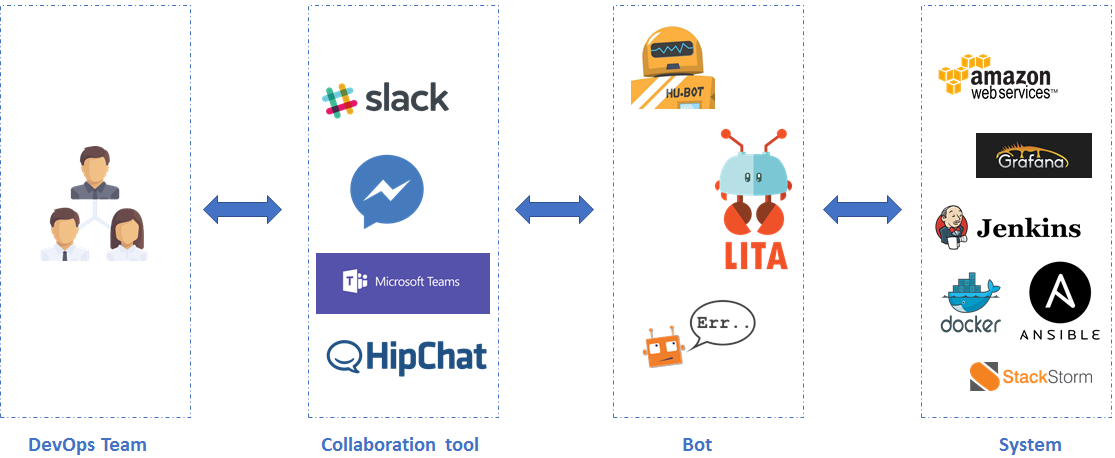
\includegraphics[width=\textwidth]{Anhang/cop}
  \quelle[o. \pno]{Zyane_2017_ChatOps}
  \caption{ChatOps Prozess}
\label{fig:cop}
\end{figure}


\subsubsection{Kollaborationswerkzeug}
Bekannte Beispiele für Kollaborationswerkzeuge sind Slack, Atlassian HipChat oder Cisco WebEx Teams, die allesamt die Integration von Bots ermöglichen.
Ziel solcher Werkzeuge ist es, Kollaboration zu ermöglichen, die Kommunikation von Arbeitsteams effektiv zu gestalten und klassische Kanäle wie E-Mail oder SMS abzulösen. Dabei ist auch die Anbindung von anderen Diensten, wie z. B. Cloud Speicher zur kollaborativen Bearbeitung von Dokumenten möglich. So müssen Unternehmen nicht zwangsläufig die Software von einem bestimmten Hersteller beziehen, sondern können das Kollaborationswerkzeug ihrer Wahl an verschiedene Dienste anbinden.
\footcites[Vgl.][o. \pno]{Zyane_2017_ChatOps}[Vgl.][o. \pno]{Koeltzsch_2019_Slack}

Slack zum Beispiel gilt als erfolgreichstes Kollaborationswerkzeug. Das Unternehmen wurde 2013 gegründet und hat heute 8 Millionen Nutzer, davon 3 Millionen zahlende und der Marktwert wird auf 7,1 Milliarden Dollar geschätzt. In der Basisversion ist es kostenlos, für Features wie längeres Vorhalten der Chatverläufe muss eine Lizenz erworben werden.
Zum Februar 2019 hat Slack den Konkurrenten HipChat abgeschaltet und die bisherigen Kunden nach Slack migriert, nachdem dieser Ende 2018 übernommen wurde.
\footcites[Vgl.][o. \pno]{Koeltzsch_2019_Slack}[Vgl.][o. \pno]{Donath_2018_Hipchat_Uebernahme}

\subsubsection{Bot}
Als ChatOps Bots können z. B. Hubot, Lita, oder  Errbot verwendet werden, wobei alle in etwa die gleiche Funktionalität besitzen, da sie sich am ursprünglichen ChatOps Bot Hubot orientieren.
Allerdings sind sie in verschiedenen Sprachen geschrieben, was für die Weiterentwicklung und Anbindung an Systeme wichtig sein kann, und weisen einige Besonderheiten auf. Eine Übersicht ist in \autoref{tab:bots} zu sehen.
\footcite[Vgl.][o. \pno]{Zyane_2017_ChatOps}

Cog hingegen ist ein Bot Framework, das möglichst plattformunabhängig arbeitet und ähnlich der Unix Funktion \textit{Pipe} funktioniert, also eine Verknüpfung verschiedener Befehle in beliebiger Komplexität ermöglicht.
\footcite[Vgl.][o. \pno]{Zyane_2017_ChatOps}

\begin{table}[H]
\centering
\begin{tabularx}{.8\textwidth}{l|l|X}
  Name & Sprache & Besonderheiten\\\hline
  Hubot & CoffeeScript & große Community\\
  Lita & Ruby & viele Plugins\\
  Errbot & Python & einfache Integration von APIs\\
  Cog & (Framework) & Unix-ähnliches Piping\\
\end{tabularx}
\quelleeigen[o. \pno]{Zyane_2017_ChatOps}
\caption{Verschiedene ChatOps Bots}
\label{tab:bots}
\end{table}

%\begin{table}[H]
%\centering
%\begin{tabularx}{1\textwidth}{|l|l|X|}\hline
%  Name & Sprache & Besonderheiten\\\hline\hline
%  Hubot & CoffeeScript & große Community\\\hline
%  Lita & Ruby & viele Plugins\\\hline
%  Errbot & Python & einfache Integration von APIs\\\hline
%  Cog & (Framework) & Unix-ähnliches Piping\\\hline
%\end{tabularx}
%\quelleeigen[o. \pno]{Zyane_2017_ChatOps}
%\caption{Verschiedene ChatOps Bots}
%\label{tab:bots}
%\end{table}

\subsubsection{Systemintegration}
Ein Chatbot kann z. B. an das Ticketsystem, Versionskontrollsystem, Konfigurationsmanagementsystem oder Monitoringsystem angebunden werden, um dort automatisiert Aufgaben auszuführen. Eine Auflistung mit Beispielen ist in \autoref{tab:integrations} zu finden.
\footcite[Vgl.][o. \pno]{Zyane_2017_ChatOps}

\begin{table}[H]
\centering
\begin{tabularx}{.8\textwidth}{l|X}
  System & Beispiele \\\hline
  Ticket& JIRA, OTRS, TeamForge \\
  Versionskontrolle & GitHub, GitLab, Bitbucket\\
  Konfigurationsmanagement & Ansible, Salt, Chef, Puppet\\
  Monitoring & Nagios, Check\_MK, Grafana, Prometheus, Kibana\\
  Continuous Integration & Jenkins, Travis CI, Bamboo\\
  \acf{IaC} & Docker, Swarm, Kubernetes, Terraform, Vagrant\\
\end{tabularx}
\quelleeigen[o. \pno]{Zyane_2017_ChatOps}
\caption{ChatOps Systemintegrationen}
\label{tab:integrations}
\end{table}

%\begin{table}[H]
%\centering
%\begin{tabularx}{1\textwidth}{|l|X|}\hline
%  System & Beispiele \\\hline\hline
%  Ticket& JIRA, OTRS, TeamForge \\\hline
%  Versionskontrolle & GitHub, GitLab, Bitbucket\\\hline
%  Konfigurationsmanagement & Ansible, Salt, Chef, Puppet\\\hline
%  Monitoring & Nagios, Check\_MK, Grafana, Prometheus, Kibana\\\hline
%  Continuous Integration & Jenkins, Travis CI, Bamboo\\\hline
%  \acf{IaC} & Docker, Swarm, Kubernetes, Terraform, Vagrant, Packer\\\hline
%\end{tabularx}
%\quelleeigen[o. \pno]{Zyane_2017_ChatOps}
%\caption{ChatOps Systemintegrationen}
%\label{tab:integrations}
%\end{table}
